\section{Architektur}

\begin{figure}[ht]
		\centering
		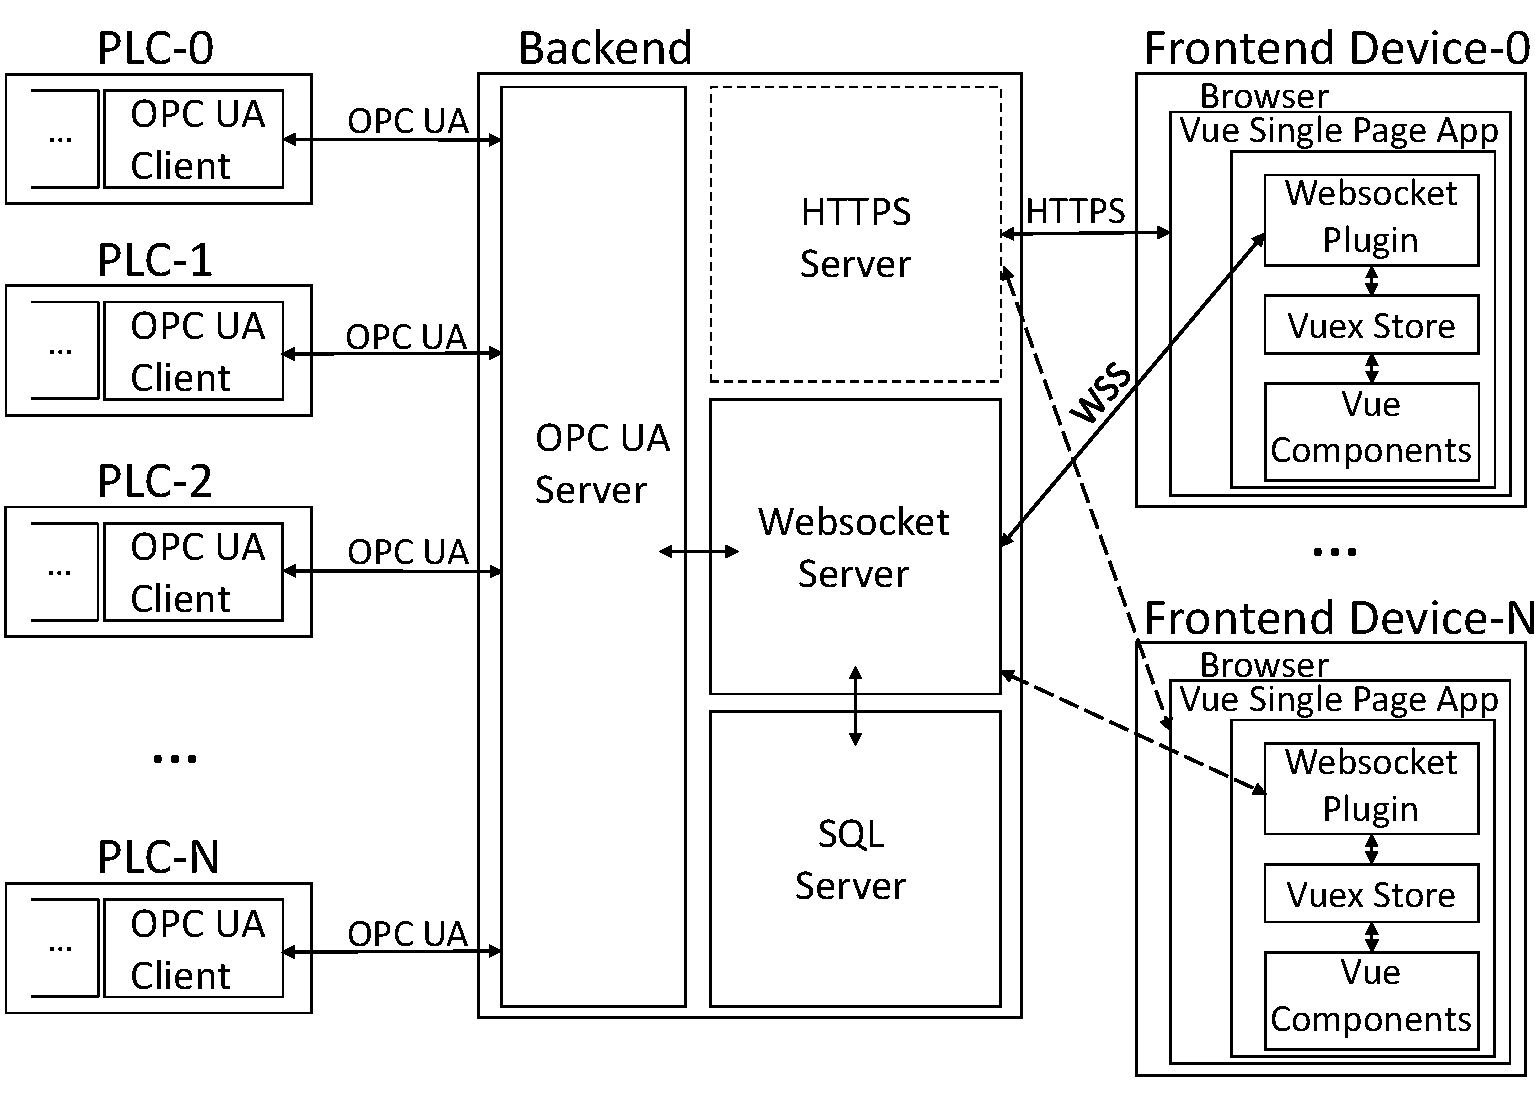
\includegraphics[width=\textwidth]{content/hauptteil/systemEntwurf/res/comMod.pdf}
    \caption[Kommunikationsmodell des \acs{scada} Systems]{Kommunikationsmodell des \acs{scada} Systems.\\
      Die CPUs sind per \acs{opcua} an das Scada System angebunden und haben die Rolle eines \acs{opcua} Clients.
      Die Webapplikation im Browser kommuniziert über \acs{wss} sowie \acs{https} verschlüsselt mit dem Backend.}
		\label{img:comMod}
\end{figure}
Wie in Abbildung \ref{img:comMod} dargestellt, lässt sich die Architektur des \ac{scada} Systems in \acp{plc}, Backend und Frontends unterteilen.
Unter Frontend (Abschnitt \ref{subsec:archFrontend}) versteht man die (in diesem Fall) grafische Schnittstelle, 
die es dem Nutzer ermöglicht mit dem System zu interagieren.
Das Backend (Abschnitt \ref{subsec:archBackend}) fasst den Rest des Systems zusammen.

\subsection{Backend}\label{subsec:archBackend}
Das Backend besteht aus den folgenden vier Komponenten:
 \begin{itemize}
  \item Einem \ac{https} Server
  \item Einem \ac{wss} Server 
  \item Einem \ac{sql} Server
  \item Einem \ac{opcua} Server 
\end{itemize}
Damit ergeben sich, wenn man das Backend von außen betrachtet, als Schnittstellen \ac{opcua}, \ac{wss} und \ac{https}.
Über diese Schnittstellen stellt das Backend den \acp{plc}, sowie dem Frontend, Services zur Verfügung.
Eine Sonderrolle unter den Komponenten nimmt dabei der \ac{https} Server ein, 
da er als einzige Komponente keine Verbindung mit dem Rest des Backends hat.
Dies ist deshalb möglich, da der \ac{https} Server dazu da ist, die \ac{html}, die \ac{css}, sowie die \ac{js} Dokumente 
einmalig beim Seitenaufruf an das Endgerät (Frontend Host Device) auszuliefern.
Von diesem Zeitpunkt an findet die Kommunikation zwischen Frontend und Backend ausschließlich über den \ac{wss} Server statt.
Dabei exist immer genau eine Session für jede Frontendinstanz.%%%
Zwischen dem Websocket Server und dem Frontend können ab diesem Zeitpunkt Strings ausgetauscht werden.
Der \ac{opcua} Server hält die variablen Daten des Systems und bietet diese den angeschlossenen \acp{plc} an.
Die Parametrierung des Frontends sowie alle anderen Daten, die persistiert werden müssen, 
werden in einem \ac{sql} Server, in Form einer relationalen Datenbank, gespeichert.

\subsection{Frontend}\label{subsec:archFrontend}
Das Frontend ist eine Webapplikation, mit Vue.js als Webframework.%unauthentifiziert->login Fenster

Beim Laden der Seite wird eine \ac{wss} Verbindung zum Backend aufgebaut.
Ohne Authentifizierung zeigt das Frontend eine Seite an, 
die es dem Nutzer ermöglicht sich durch individuelle Zugansdaten (Benutzername und Passwort) zu authentifizieren. %authentifiziert->layout fig
Werden auf dieser Seite gültige Zugangsdaten eingegeben, ist die \ac{wss} Session authentifiziert und 
zeigt das Layout in Abbildung \ref{fig:pageLayoutFrontendAuthenticated} an.
\begin{figure}[ht]
  \centering
  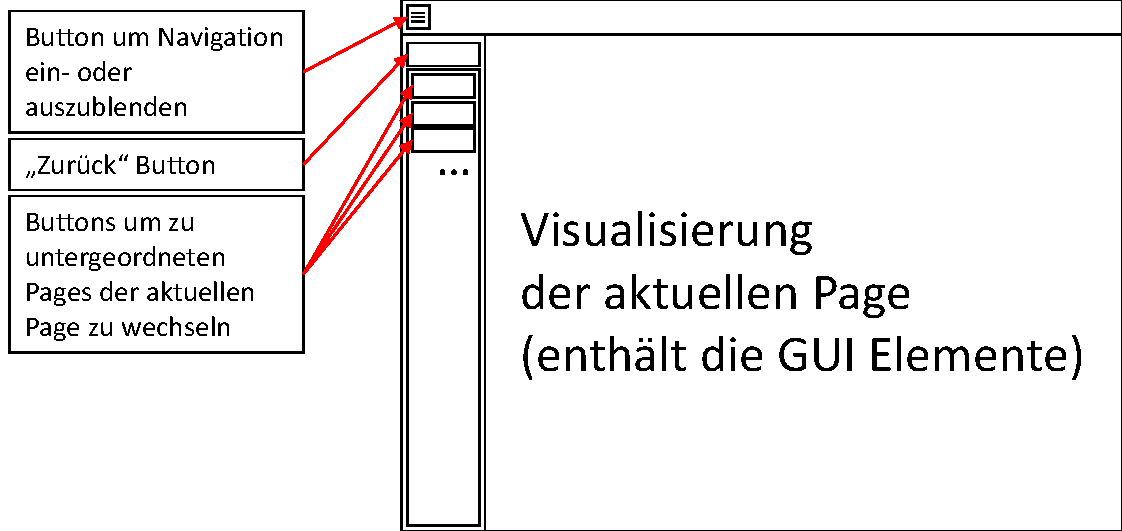
\includegraphics[width=\textwidth]{content/hauptteil/systemEntwurf/res/LayoutFrontend.pdf}
  \caption[Frontend Layout]{Layout des Frontends bei einer authentifizierten \acs{wss} Session}
  \label{fig:pageLayoutFrontendAuthenticated}
\end{figure}
Das Layout beinhaltet oben links einen Button um die Navigation der Seite ein und auszublenden.
Ist die Navigation am linken Rand eingeblendet, so ermöglicht sie es zwischen den einzelnen Seiten der Visualisierung zu navigieren.
Dazu zeigt die Navigation immer einen \glqq{}Zurück'' Button, um in die übergeordnete Seite zu wechseln, sowie Buttons um zu den untergeordneten Seiten zu wechseln.
Existieren keine untergeordneten Seiten, oder keine übergeordnete Seite, so existieren auch die Buttons nicht.
Schließlich wird im zentralen Fenster die aktuelle Page der Visualisierung angezeigt.
Der komplette Seiteninhalt ist eine Repräsentation des Datenobjekts, das global in der Webapplikation vorliegt.
Diese Datenstruktur ist eine Kopie der Daten aus dem Backend (Abschnitt \ref{subsec:dataBackend}), welche die aktuell angezeigte Seite betreffen.
Sie ist in Abschnitt \ref{subsec:dataFrontend} genauer beschrieben und kann nur über die Websocket Schnittstelle verändert werden. 
So ist sichergestellt, dass die \ac{gui} Elemente immer die Daten des Backends darstellen und es keine Unterschiede gibt.
Der Zustand ist also über alle Instanzen des Backends und Frontends immer konsistent.
Wie Daten verändert werden können ist genauer in Abschnitt \ref{subsec:protokollBackendFrontend} beschrieben.
Innerhalb der Webapplikation existiert eine Page Komponente die, entsprechend der \ac{gui} Elemente in der globalen Datenstruktur, 
\ac{gui} Element Komponenten (\emph{guiElement}) instanziert und auf der Page anzeigt.
Diese \ac{gui} Elemente werden entsprechend ihres Typs (zum Beispiel \emph{Button}) weiter in spezialisierte \ac{gui} Elemente (z.B. \emph{guiElementButton}) unterteilt.
Das Schema, wie innerhalb der Webapplikation auf Daten zugegriffen werden kann, bzw. Daten geändert werden können,
ist in Abbildung \ref{fig:dataFlowFrontend} dargestellt.
Die \ac{gui} Elemente haben nun Zugriff auf eine Funktion um Datenänderungen anzufordern, 
sowie auf den ihnen zugeordneten Teil der globalen Datenstruktur.
\begin{figure}[ht]
  \centering
  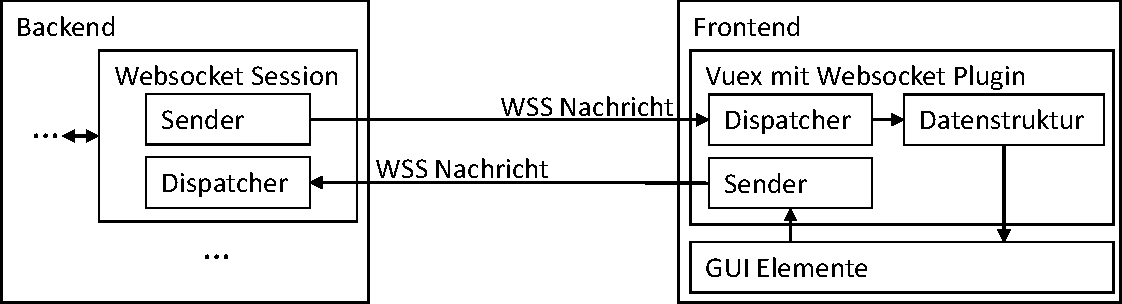
\includegraphics[width=\textwidth]{content/hauptteil/systemEntwurf/res/datenzugriffFrontend.pdf}
  \caption[Datenzugriff innerhalb des Frontends]{Schema des Zugriffs auf die Datenstruktur des Frontends}
  \label{fig:dataFlowFrontend}
\end{figure}
Wie der Dispatcher die Struktur des Frontends ändert ist in Abschnitt \ref{subsec:protokollBackendFrontend} beschrieben.
Die \ac{gui} Elemente können nur lesend auf die Datenstruktur zugreifen.


\subsection{Protokoll zwischen Frontend und Backend}\label{subsec:protokollBackendFrontend}
Websockets bieten die Möglichkeit asynchron Daten zwischen Frontend und Backend auszutauschen, 
bieten allerdings keinerlei Regeln für die Semantik dieser Daten. 
Deshalb ist ein weiteres Protokoll in der Applikationsebene erforderlich, 
welches die Semantik der ausgetauschten Daten definiert. 
An dieses Protokoll werden folgende Anforderungen gestellt.\\
Das Protokoll soll
\begin{itemize}
 \item [\dots]so einfach wie möglich sein.
 \item [\dots]alle Datentypen unterstützen, die das Backend definiert.
 \item [\dots]weitestgehend symmetrisch sein (Die Nachrichten vom Server zum Client haben eine ähnliche Gestalt wie die vom Client zum Server).
 \item [\dots]möglichst leichtgewichtig sein.
 \item [\dots]möglichst frei von Zuständen sein, sodass ein Vertauschen zweier Nachrichten keine Relevanz für die Applikation darstellt.
 \item [\dots]eine Authentifizierung des Nutzers ermöglichen.
\end{itemize}
Die meisten Anforderungen können erfüllt werden, allerdings stehen die letzten drei in Konkurrenz zueinander.
Um eine Authentifizierung zu ermöglichen gibt es, bei einer Verbindung die ab dem Aufbau dauerhaft besteht, folgende Möglichkeiten:
\begin{itemize}
  \item Die Zugangsdaten, die die Session authentifizieren, werden einmalig vom Client zum Server gesendet.
  Die Session ist dann authentifiziert und hat ab diesem Zeitpunkt mehr Rechte.
  \item Die Zugangsdaten werden bei jeder Nachricht mitgesendet und überprüft. 
\end{itemize}
Die erste Variante ist möglichst leichtgewichtig, da die Zugangsdaten nur einmal gesendet werden. 
Allerdings ist sie nicht frei von Zuständen, da die Schnittstelle, je nachdem ob eine Session bereits authentifiziert ist, unterschiedlich auf eingehende Nachrichten reagiert.
Die zweite Variante reagiert immer identisch (deterministisch) auf die gleiche Nachricht, 
ist aber weniger performant, da das Verhältnis von Protokoll-Overhead zu Nutzdaten immer größer ist als bei der ersten Variante.
Aufgrund dieses Sachverhalts wird bei der Zustandsfreiheit eine Ausnahme gemacht werden.\\
\begin{figure}[ht]
  \centering
  \begin{subfigure}[b]{0.601833561\textwidth}
    \includegraphics[width=\textwidth]{content/hauptteil/systemEntwurf/res/protokoll/ws_Message.pdf}
    \caption{Websocket Message Container mit \\ \emph{event} (Header) und \emph{payload} (Nutzdaten)}
    \label{fig:CDWME:ws_message}
  \end{subfigure}
  \hfill
  \begin{subfigure}[b]{0.388166439\textwidth}
    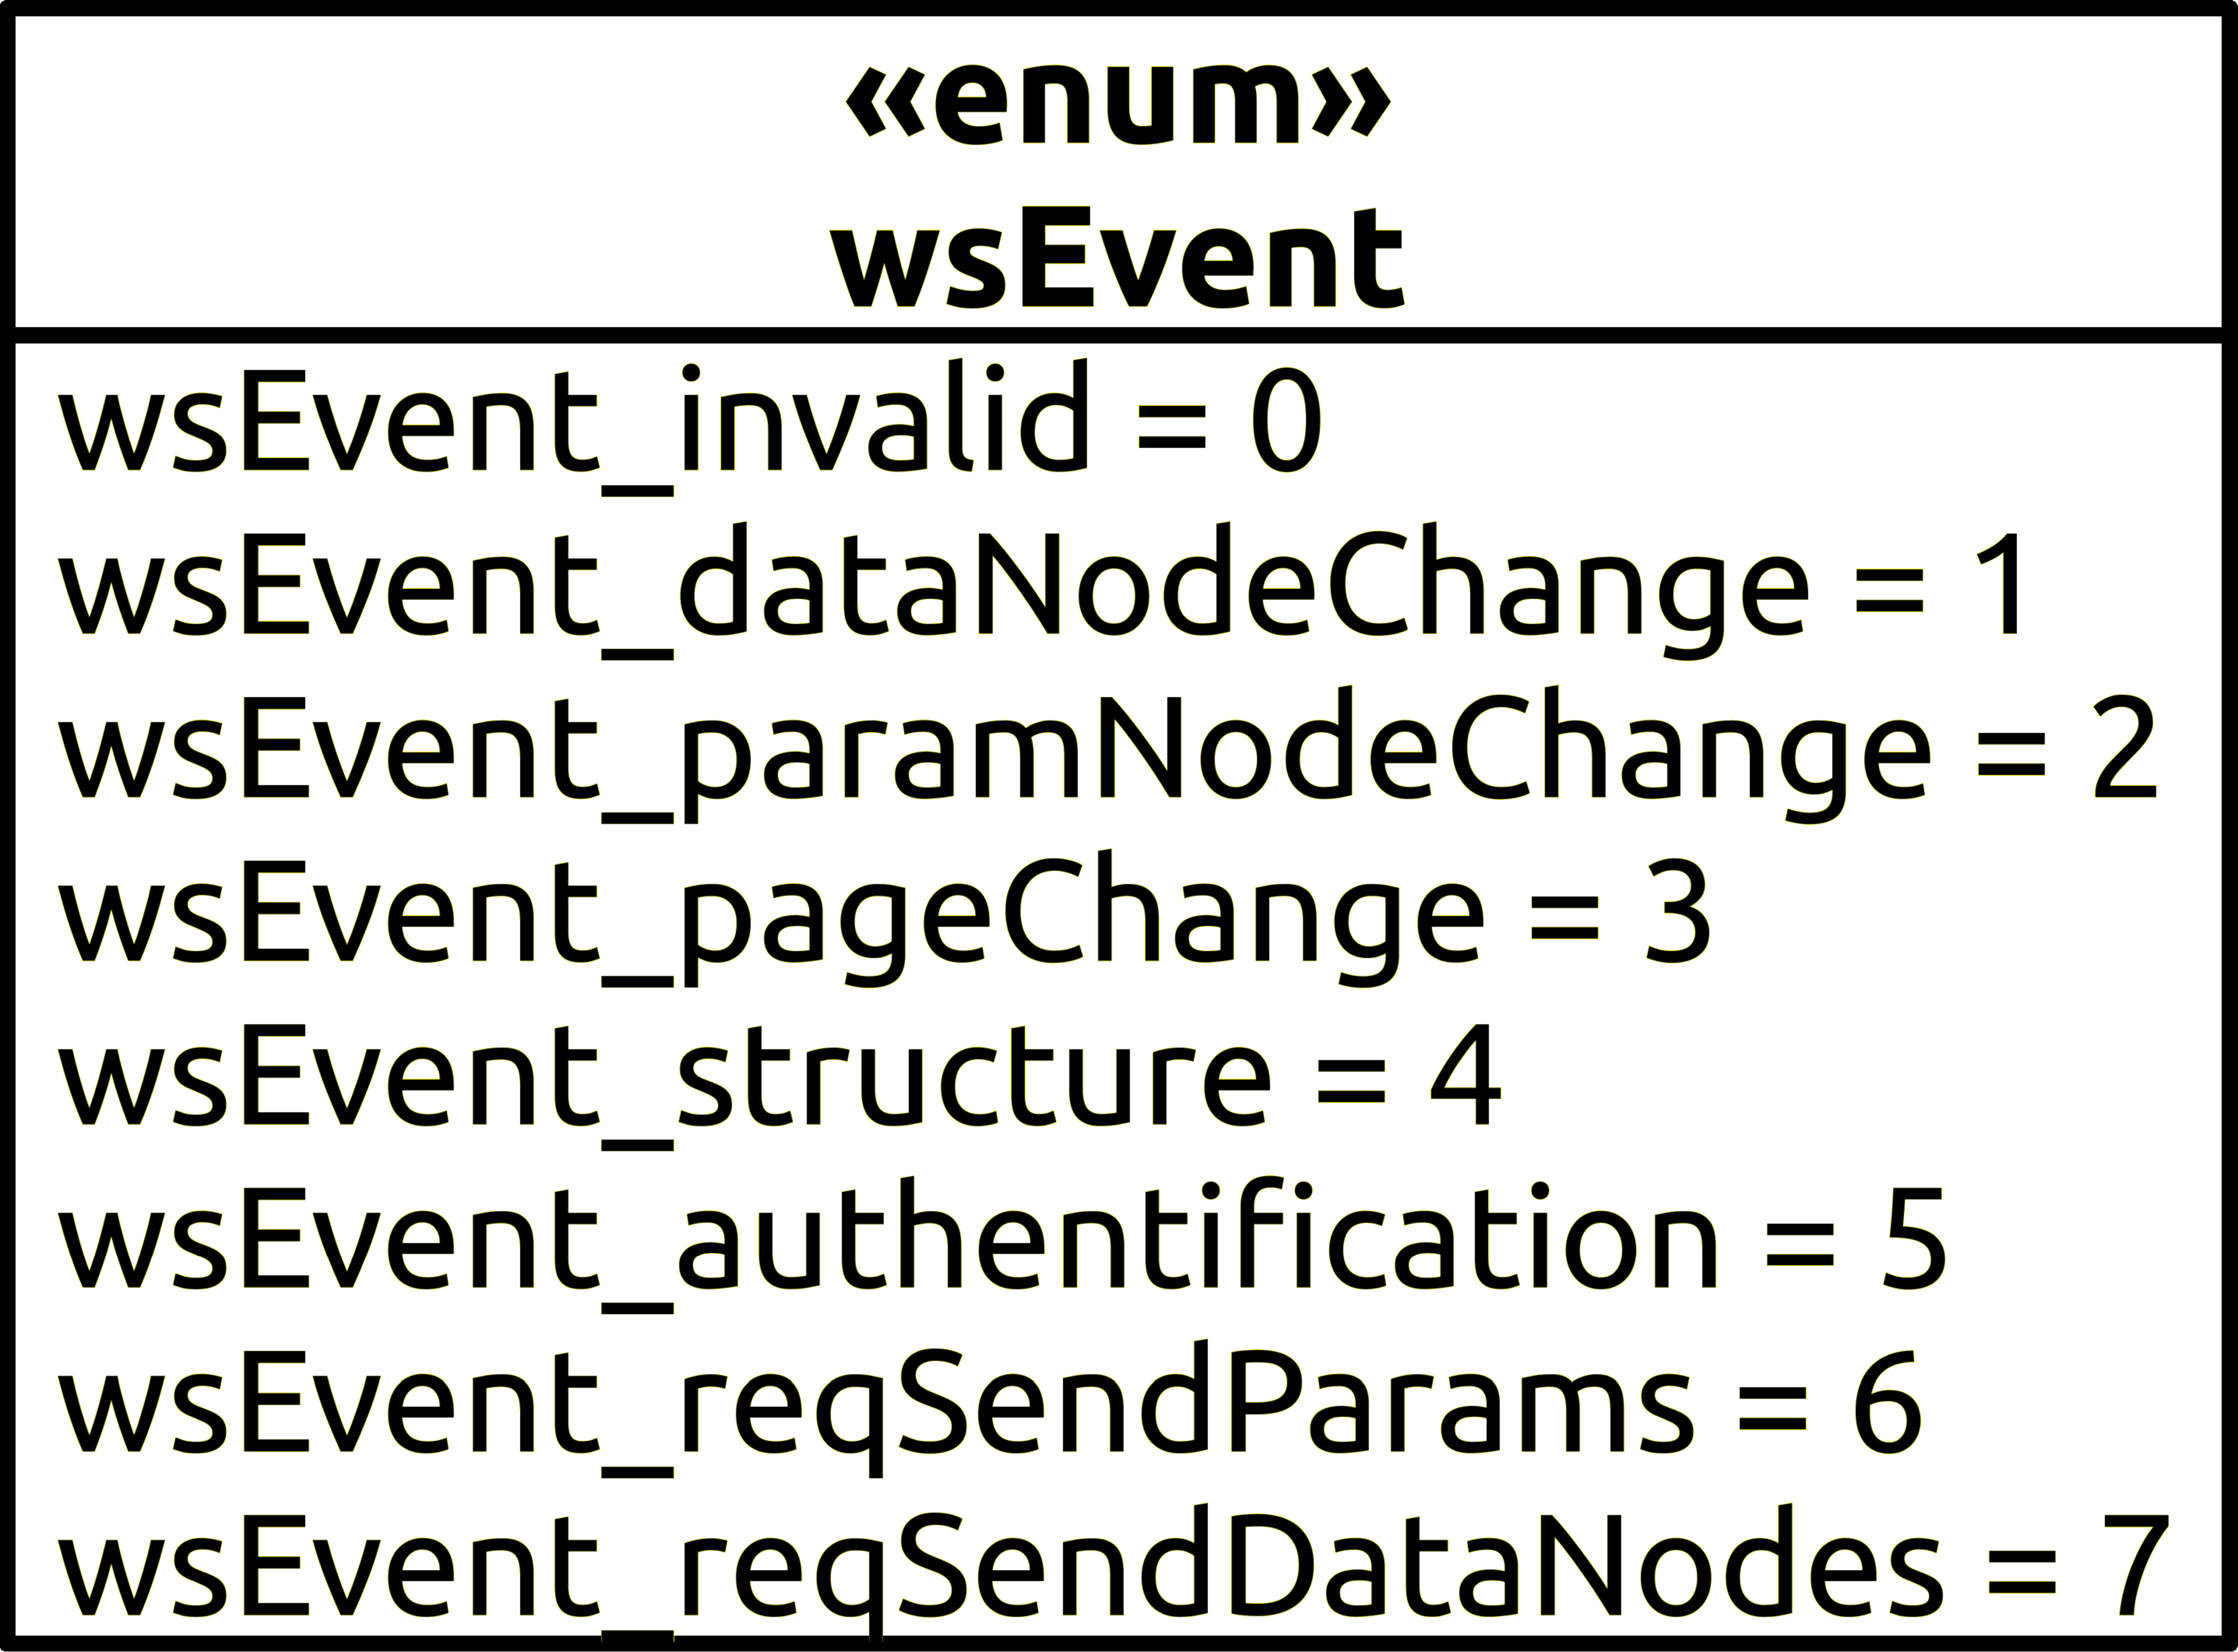
\includegraphics[width=\textwidth]{content/hauptteil/systemEntwurf/res/protokoll/wsEvent.pdf}
    \caption{Websocket Event Definition als Aufzählung}
    \label{fig:CDWME:wsEvent}
  \end{subfigure}
  \caption[Websocket Message Container und Event]{Websocket Message Container und Event}
  \label{fig:CDWME}
\end{figure}
Das erarbeitete Protokoll tauscht Strings aus, dessen Struktur der Klasse in Abbildung \ref{fig:CDWME:ws_message} zugrunde liegt.
Diese Klasse besteht aus Nutzdaten (\emph{payload}), sowie einem Header (\emph{event}).
Nutzdaten sind nur optional vorhanden, so ist möglich nur ein Event zu verschicken.
Der Header ist eine Aufzählung verschiedener Events. 
Diese Aufzählung (\emph{wsEvent}) ist in Abbildung \ref{fig:CDWME:wsEvent} dargestellt und gibt die einzelnen Typen von Nachrichten an. 
Ein solches Objekt kann seitens des Backends aus dem String in einer Websocket Nachricht konstruiert, 
sowie in einen solchen String übersetzt werden. 
Die Bildungsvorschrift ist dabei, alle Information welche das \emph{ws\_message} Objekt enthält (\emph{event} und \emph{payload}), als String zu kodieren 
und durch ein Semikolon getrennt zu einem String zusammenzusetzen.
Dabei stellt das erste Feld in einem versendeten String immer das kodierte Event dar. Die restlichen Felder entsprechen dem Nutzdatenvektor der \emph{ws\_message}.
Diese Bildungsvorschrift ist umkehrbar, solange der Nutzdatenvektor kein String mit einem Semikolon enthält.
Dieser Fall ist unbedingt zu vermeiden und muss vom Frontend und Backend beim Kodieren des Strings abgefangen werden.
Die umgekehrte Bildungsvorschrift implementiert die \emph{ws\_message} Klasse als Konstruktor. 
Das Protokoll unterstützt nun die in Abbildung \ref{fig:CDWME:wsEvent} dargestellten Events.
Das erste Event (\emph{wsEvent\_invalid}) ist der Standartwert des Events in jedem \emph{ws\_message} Objekt. 
Auf eine Nachricht mit diesem Event wird beim Empfang von keiner Seite aus reagiert und die Nachricht verworfen.
Dies ist eine Absicherung, um zu verhindern, dass eine Nachricht mit einem zufälligen Event versendet wird.
Front- sowie Backend stellen einen Dispatcher zur Verfügung welcher, entsprechend des Events einer empfangenen Nachricht, einen Handler aufruft.
Der Dispacher des Backends unterscheidet sich vom Dispatcher im Frontend, da er die Authentifizierung des Nutzers realisiert.
Das Verhalten, ob und wie eine Nachricht vom Dispatcher im Backend dispatcht wird, 
ist durch das Aktivitätsdiagramm in Abbildung \ref{fig:aDDB:entry} definiert.
Hier werden nur Nachrichten dispatcht, wenn die Websocketsession bereits authentifiziert wurde oder die Nachricht eine Authentifizierungsnachricht ist.
Ist dies der Fall, werden die entsprechenden Handler zu den empfangenen Events aufgerufen.
%Diese Handler sind:
%\begin{itemize}
%  \item wsEvent\_structure (Abbildung \ref{fig:aDDB:wsEvent_structure})
%  \item wsEvent\_authentification (Abbildung \ref{fig:aDDB:wsEvent_authentification})
%  \item wsEvent\_dataNodeChange (Abbildung \ref{fig:aDDB:wsEvent_dataNodeChange})
%  \item wsEvent\_paramNodeChange (Abbildung \ref{fig:aDDB:wsEvent_paramNodeChange})
%  \item wsEvent\_reqSendParamNodes (Abbildung \ref{fig:aDDB:wsEvent_reqSendParamNodes})
%  \item wsEvent\_reqSendDataNodes (Abbildung \ref{fig:aDDB:wsEvent_reqSendDataNodes})
%  \item wsEvent\_pageChange (Abbildung \ref{fig:aDDB:wsEvent_pageChange})
%\end{itemize}

Die Handler des Backends sind durch die verbleibenden Diagramme in Abbildung \ref{fig:activityDiagramDispatcherBackendI}, 
sowie durch die Diagramme in Abbildung \ref{fig:activityDiagramDispatcherBackendII} definiert.
Die Handler des Frontends sind in Abbildung \ref{fig:activityDiagramDispatcherFrontend} dargestellt.

Das Frontend bedarf keines solchen Authentifizierungsmechanismus, da dies bereits im \ac{wss} Protokoll implementiert ist. 
Wie auch bei \ac{https} geschieht das durch ein Serverzertifikat des Backends, 
dass durch eine externe \ac{ca} beim Verbindungsaufbau verifiziert werden muss.
Das Fro
%hier weite auf handler eingehn und wie die kommunikation zwischen vuex und ws funktioniert.

%Der Weg, Daten zu verändern ist nun, mit einer Nachricht an das Backend eine Datenänderung \glqq{}anzufragen''.
%Ist die Änderung möglich, Sendet der Server
\begin{figure}[ht]
  \centering
  \begin{subfigure}[b]{0.66222973\textwidth}
    \centering
    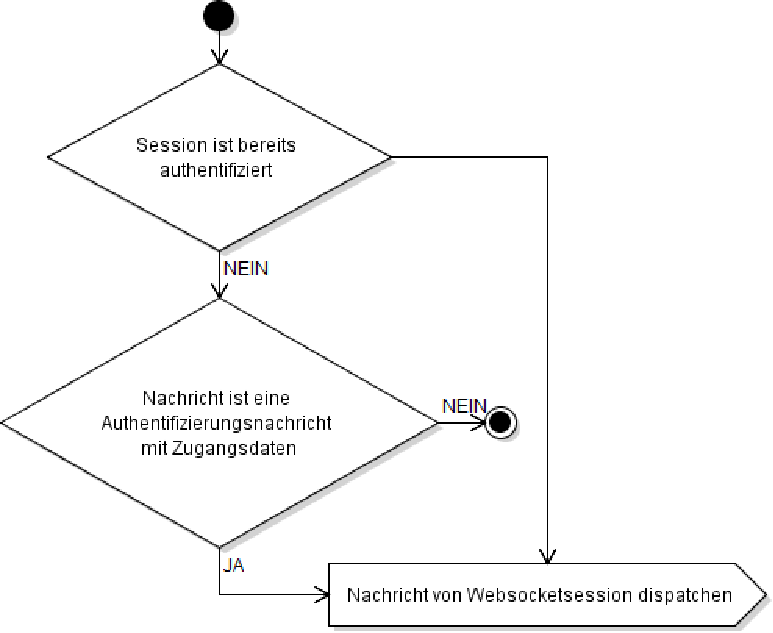
\includegraphics[width=\textwidth]{content/hauptteil/systemEntwurf/res/wsHandler/backend/message_received.pdf}
    \caption{WebsocketEvent empfangen}
    \label{fig:aDDB:entry}
  \end{subfigure}
  \hfill
  \begin{subfigure}[b]{0.32777027\textwidth}
    \centering
    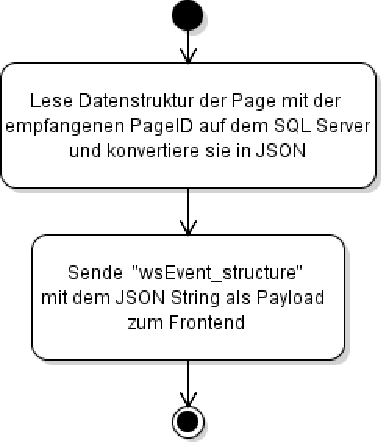
\includegraphics[width=\textwidth]{content/hauptteil/systemEntwurf/res/wsHandler/backend/wsEvent_structure.pdf}
    \caption{WebsocketEvent:\\\emph{Structure} empfangen}
    \label{fig:aDDB:wsEvent_structure}
  \end{subfigure}
  \hspace{50mm}

  \begin{subfigure}[b]{0.406343284\textwidth}
    \centering
    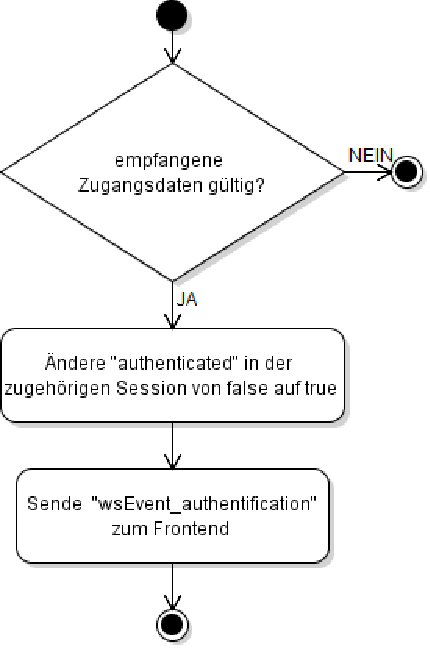
\includegraphics[width=\textwidth]{content/hauptteil/systemEntwurf/res/wsHandler/backend/wsEvent_authentification.pdf}
    \caption{WebsocketEvent:\\\emph{Authentification} empfangen}
    \label{fig:aDDB:wsEvent_authentification}
  \end{subfigure}
  \hfill
  \begin{subfigure}[b]{0.583656716\textwidth}
    \centering
    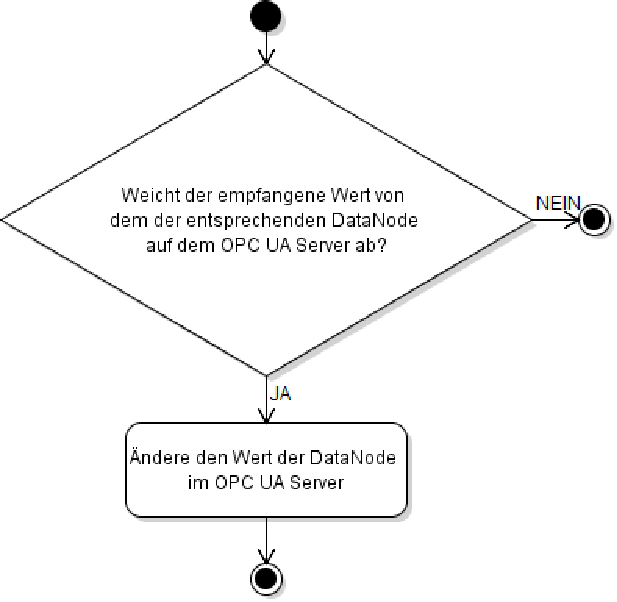
\includegraphics[width=\textwidth]{content/hauptteil/systemEntwurf/res/wsHandler/backend/wsEvent_dataNodeChange.pdf}
    \caption{WebsocketEvent:\\\emph{DataNodeChange} empfangen}
    \label{fig:aDDB:wsEvent_dataNodeChange}
  \end{subfigure}

  \caption[Aktivitätsdiagramme Dispatcher Backend I]{Aktivitätsdiagramme des Dispatchers im Backend I}
  \label{fig:activityDiagramDispatcherBackendI}
\end{figure}

  
\begin{figure}[ht]
  \centering
   \begin{subfigure}[b]{0.543125\textwidth}
    \centering
    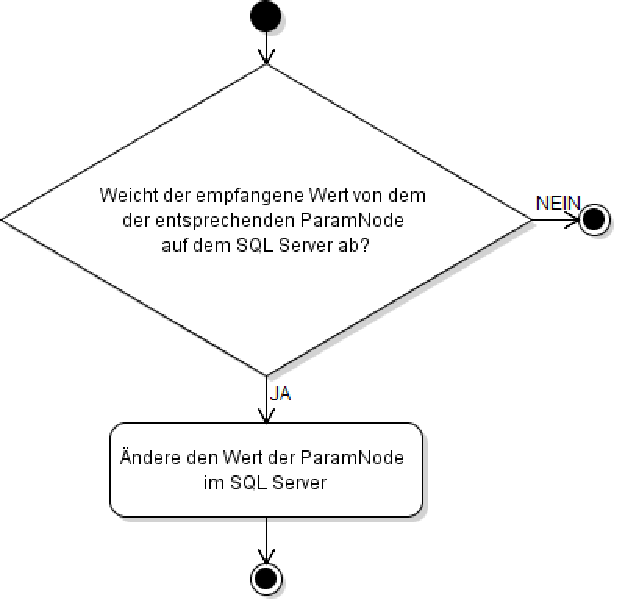
\includegraphics[width=\textwidth]{content/hauptteil/systemEntwurf/res/wsHandler/backend/wsEvent_paramNodeChange.pdf}
    \caption{WebsocketEvent:\\\emph{ParamNodeChange} empfangen}
    \label{fig:aDDB:wsEvent_paramNodeChange}
  \end{subfigure}
  \hfill
  \begin{subfigure}[b]{0.446875\textwidth}
    \centering
    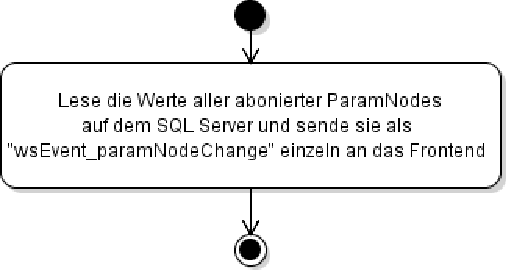
\includegraphics[width=\textwidth]{content/hauptteil/systemEntwurf/res/wsHandler/backend/wsEvent_reqSendParamNodes.pdf}
    \caption{WebsocketEvent:\\\emph{ReqSendParamNodes} empfangen}
    \label{fig:aDDB:wsEvent_reqSendParamNodes}
  \end{subfigure}
  \hspace{50mm}

  \begin{subfigure}[b]{0.4875\textwidth}
    \centering
    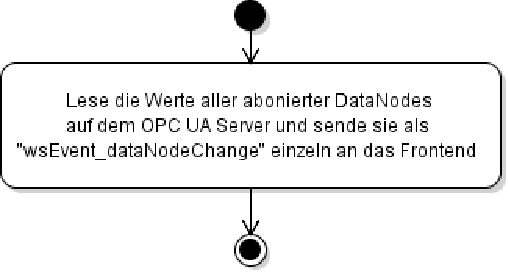
\includegraphics[width=\textwidth]{content/hauptteil/systemEntwurf/res/wsHandler/backend/wsEvent_reqSendDataNodes.pdf}
    \caption{WebsocketEvent:\\\emph{ReqSendDataNodes} empfangen}
    \label{fig:aDDB:wsEvent_reqSendDataNodes}
  \end{subfigure}
  \hfill
  \begin{subfigure}[b]{0.5025\textwidth}
    \centering
    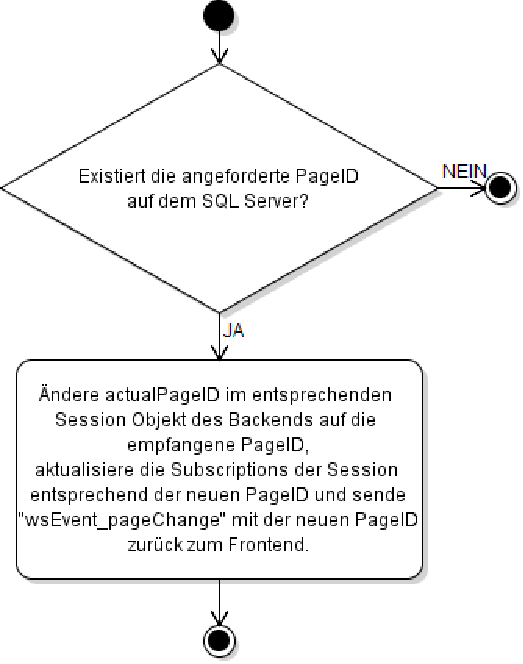
\includegraphics[width=\textwidth]{content/hauptteil/systemEntwurf/res/wsHandler/backend/wsEvent_pageChange.pdf}
    \caption{WebsocketEvent:\\\emph{PageChange} empfangen}
    \label{fig:aDDB:wsEvent_pageChange}
  \end{subfigure}
  \caption[Aktivitätsdiagramm Dispatcher Backend II]{Aktivitätsdiagramme des Dispatchers im Backend II}
  \label{fig:activityDiagramDispatcherBackendII}
\end{figure}

\begin{figure}[ht]
  \centering
  \begin{subfigure}[b]{0.48\textwidth}
    \centering
    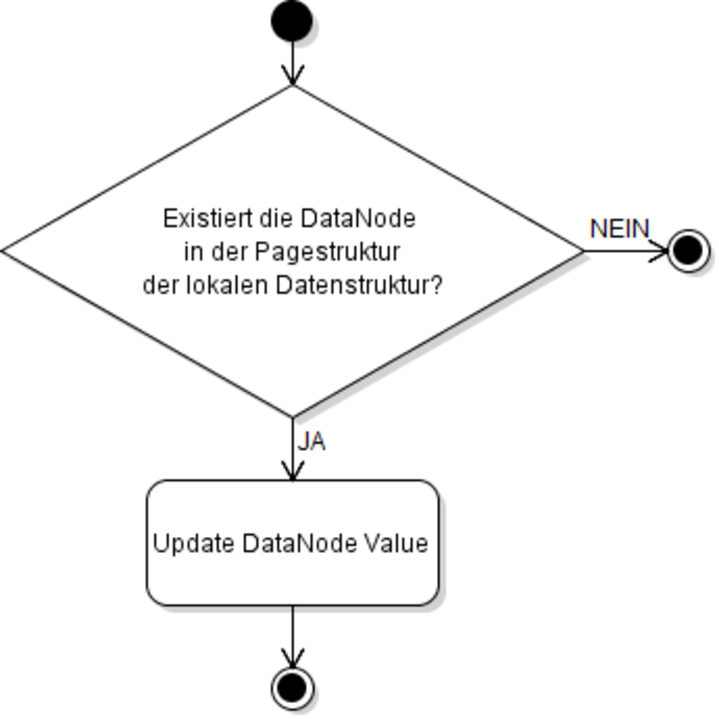
\includegraphics[width=\textwidth]{content/hauptteil/systemEntwurf/res/wsHandler/frontend/wsEvent_dataNodeChange.pdf}
    \caption{WebsocketEvent:\\\emph{DataNodeChange} empfangen}
    \label{fig:aDDF:wsEvent_dataNodeChange}
  \end{subfigure}
  \hfill
  \begin{subfigure}[b]{0.48\textwidth}
      \centering
      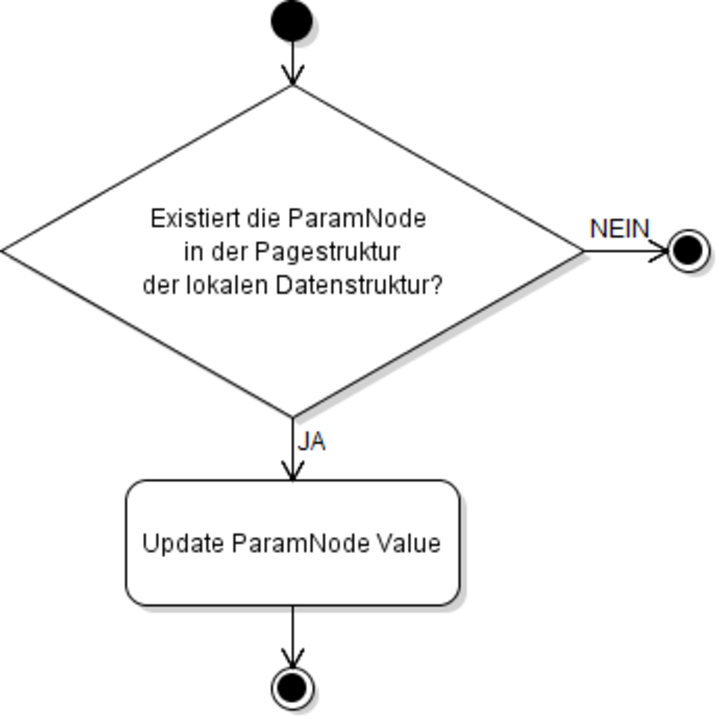
\includegraphics[width=\textwidth]{content/hauptteil/systemEntwurf/res/wsHandler/frontend/wsEvent_paramNodeChange.pdf}
      \caption{WebsocketEvent:\\\emph{ParamNodeChange} empfangen}
      \label{fig:aDDF:wsEvent_paramNodeChange}
  \end{subfigure}
  \hspace{50.00mm}

  \begin{subfigure}[b]{0.3\textwidth}
      \centering
      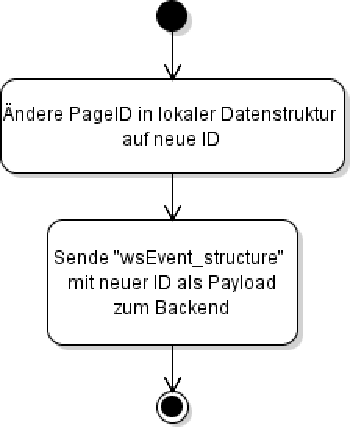
\includegraphics[width=\textwidth]{content/hauptteil/systemEntwurf/res/wsHandler/frontend/wsEvent_pageChange.pdf}
      \caption{WebsocketEvent:\\\emph{PageChange} empfangen}
      \label{fig:aDDF:wsEvent_pageChange}
  \end{subfigure}
  \hfill
  \begin{subfigure}[b]{0.38\textwidth}
      \centering
      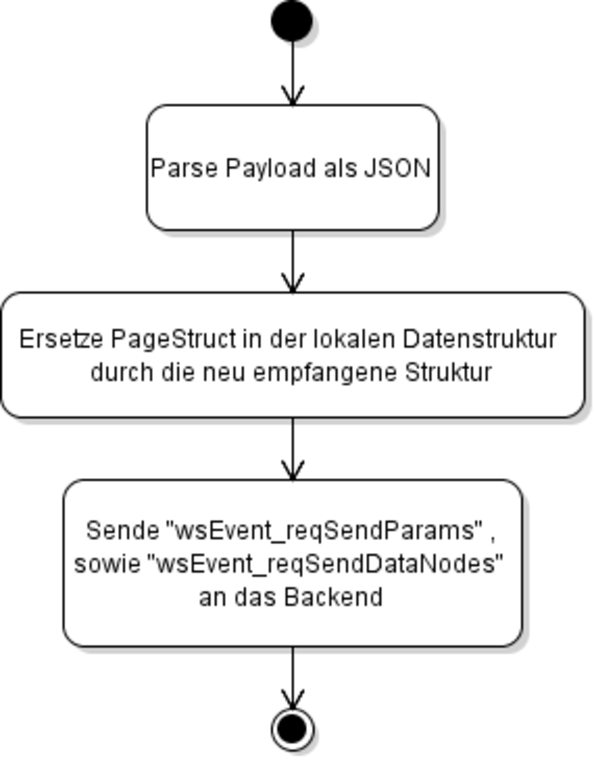
\includegraphics[width=\textwidth]{content/hauptteil/systemEntwurf/res/wsHandler/frontend/wsEvent_structure.pdf}
      \caption{WebsocketEvent:\\\emph{Structure} empfangen}
      \label{fig:aDDF:wsEvent_structure}
  \end{subfigure}
  \hfill
  \begin{subfigure}[b]{0.30\textwidth}
      \centering
      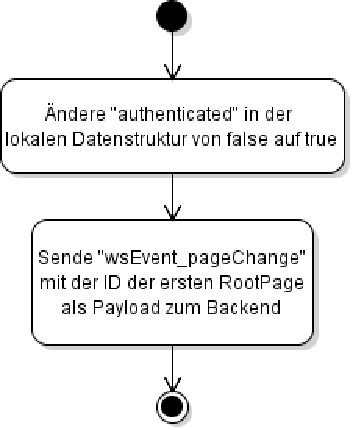
\includegraphics[width=\textwidth]{content/hauptteil/systemEntwurf/res/wsHandler/frontend/wsEvent_authentification.pdf}
      \caption{WebsocketEvent:\\\emph{Authentification} empfangen}
      \label{fig:aDDF:wsEvent_authentification}
  \end{subfigure}
     \caption[Aktivitätsdiagramme Dispatcher Frontend]{Aktivitätsdiagramme des Dispatchers im Frontend}
     \label{fig:activityDiagramDispatcherFrontend}
\end{figure}
asdasd
\section{Datenstruktur}
\subsection{Backend}\label{subsec:dataBackend}
\begin{figure}[ht]
  \centering
  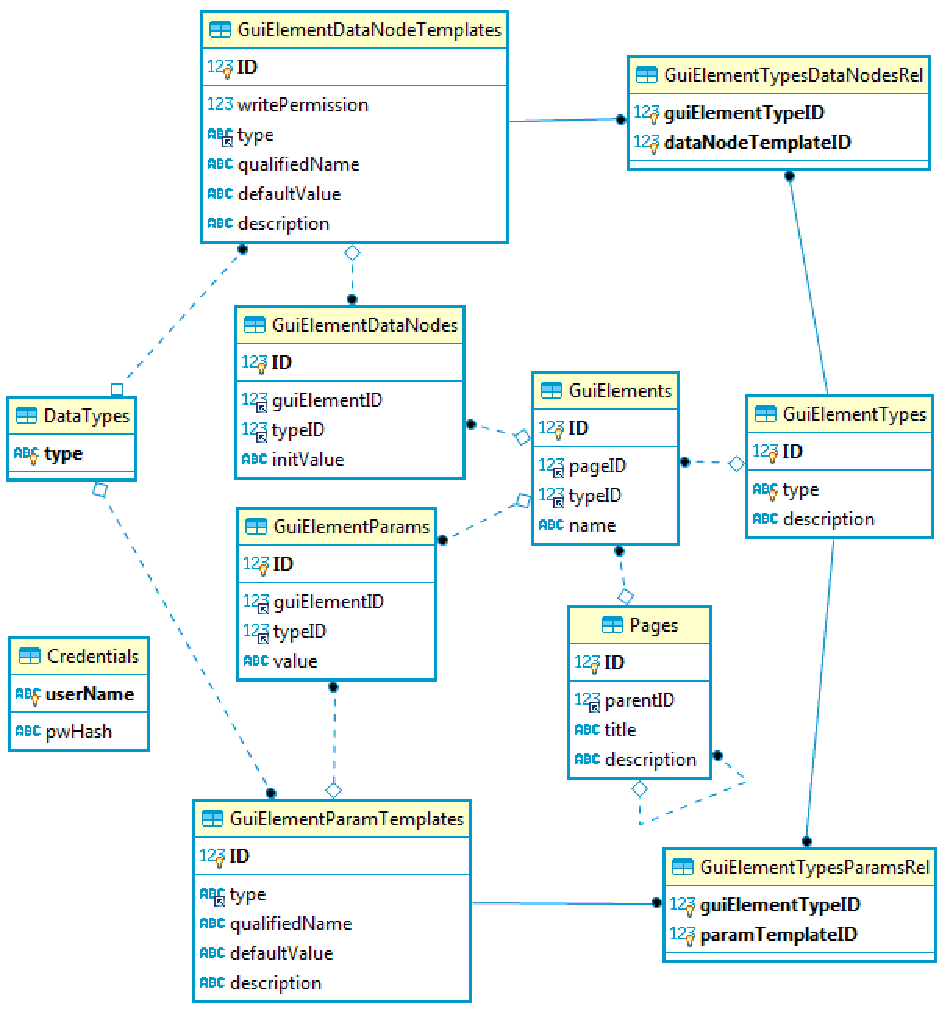
\includegraphics[width=\textwidth]{content/hauptteil/systemEntwurf/res/erd.pdf}
  \caption[\acs{erd} des \acs{scada} Systems]{\acs{erd} des \ac{scada} Systems.\\
    Darstellung zeigt die einzelnen Tabellen der Datenbank auf dem \ac{sql} Server und deren Beziehungen zueinander.}
  \label{img:erd}
\end{figure}
Das abgebildete \ac{erd} in Abbildung \ref{img:erd}, stellt die globale Datenstruktur der Datenbank auf dem \ac{sql} Server dar.
Sie besteht aus einzelnen Tabellen deren Primärschlüssel, ausgenommen einzelner Hilfstabellen, immer eine ID ist.
Zentrales Element sind dabei die \ac{gui} Elemente (Tabelle \emph{GuiElements}). Jedes \ac{gui} Element ist einer Page (Tabelle \emph{Pages}) zugeordnet. 
Eine Page kann wiederum einer anderen Page zugeordnet sein. 
Dies wird erreicht indem jeder Page-Datensatz eine ParentID enthält, welche als Fremdschlüssel auf die übergeordnete Page zeigt. So entsteht eine Baumstruktur innerhalb der Entitäten.
Ist der Wert dieses Fremdschlüssels \emph{NULL} so hat die jeweilige Page keine übergeordnete Page und liegt damit im Wurzelverzeichnis.\\
Jedes \ac{gui} Element hat \emph{n} Parameter und \emph{m} Data Nodes (mit $ n, m \in \N $). 
Diese werden in den Tabellen \emph{GuiElementParams} sowie \emph{GuiElementDataNodes} verwaltet.
Jede DataNode, beziehungsweise jeder Parameter, hat einen Datentyp, einen Namen, eine Beschreibung, sowie einen Wert. 
Bei den Parametern entspricht dies dem tatsächlichen aktuellen Wert, 
bei den DataNodes entspricht dies dem initialen Wert beim Starten des Backends.
Die zuvor beschriebenen \ac{gui} Elemente besitzen außerdem einen Typ (verwaltet in der Tabelle \emph{GuiElementTypes}).
Jedem Typ sind nun \emph{n} DataNodeTemplates (Tabelle \emph{GuiElementDataNodeTemplates}) zugeordnet, 
aus denen die eigentlichen DataNodes beim Instanzieren erstellt werden. Da eine solche Vorlage für DataNodes auch für mehrere \ac{gui} Element Typen verwendet werden kann, 
ist die Verbindung eine $n:m$ Bindung. 
Dies ist in einer Datenbank nur durch eine Hilfstabelle, 
welche die Primärschlüssel zweier Tabellen miteinander verknüpft, ereichbar. 
Analog zu den DataNodes ist der gleiche Mechanismus für die Parameter vorgesehen.
Um ein sauberes Interface zu schaffen sind zum Instanzieren, 
sowie zum Löschen der \ac{gui} Elemente, Stored Procedures vorgesehen.
Die komplette Datenstruktur des \ac{sql} Servers ist so abgelegt, 
dass dieser alle relevanten Relationen kennt und entsprechend verwaltet.
So werden beispielsweise beim Löschen eines \ac{gui} Elements alle zugehörigen DataNodes mitgelöscht und 
beim Löschen einer kompletten Page werden alle der Page zugeordneten \ac{gui} Elemente auch gelöscht (\emph{on delete cascade}, Abschnitt \ref{subsec:relDB}).\\ \\

Der \ac{opcua} Server hält alle DataNodes der \ac{gui} Elemente. 
Diese \ac{gui} Elemente werden entsprechen der Pages, denen sie zugeordnet sind, auf dem \ac{opcua} Server abgelegt und 
sind den \acp{plc} dort zugänglich.
Ob eine DataNode von den \acp{plc} nur gelesen oder auch beschrieben werden kann, 
wird durch das Flag \emph{writePermission} auf dem \ac{sql} Server in der \emph{DataNodeTemplate} Tabelle festgelegt. 
Beim Erstellen der DataNode auf dem \ac{opcua} Server, wird dieses Flag ausgelesen und 
direkt in die Konfiguration des \ac{opcua} Servers übernommen.
Der native Datentyp, mit dem eine DataNode auf dem \ac{opcua} Server abgelegt wird, wird den DataNodeTemplates des \ac{sql} Servers entnommen.

Auf dem \ac{sql} Server haben die DataNodes, sowie Parameter, immer den nativen \ac{sql} Datentyp \emph{VARCHAR}, um ein Speicherfeld zu erhalten, das alle benutzten \ac{opcua} Datentypen unterstützt.
Beim Lesen, beziehungsweise beim Schreiben, wird der als String gespeicherte Wert auf dem \ac{sql} Server, 
entsprechend seines explizit abgespeicherten Datentyps, konvertiert. 
%hier noch mehr entry: OPCUASERVER::createDataNode(MYSQL_RES) aber: abstract ohne auf impl einzugehn
GuiElements und Pages haben als Datentyp auf dem \ac{opcua} Server den Typ BaseObjectType.
Auf einen Spezialisierung dieser Typdefinition für Pages und \ac{gui} Elements auf dem \ac{opcua} Server wird absichtlich verzichtet, 
da sie nur zur Strukturierung der DataNodes, auf dem \ac{opcua} Server, genutzt werden.


\subsection{Frontend}\label{subsec:dataFrontend}
\dots



